\section{Abstract Syntax}
编程语言 = 语法(识别一个合法的程序) + 语义(这个合法的程序对应的实际行为)


\subsection{Attribute Grammar(属性文法)}
属性文法=上下文无关文法+属性+属性计算规则
\begin{itemize}
    \item 属性: 描述文法符号的语义特征
    \item 属性计算规则(语义规则): 表明属性间``抽象''关系
\end{itemize}

\subsection{Semantic Action(语义动作)}
给产生式绑定一个语义动作, 使得按照这个产生式规约时/推导时完成特定操作. 

\subsection{Abstract Parse Tree(抽象解析树)}
叶节点对应输入的token, 内部节点对应一个语法规则. 

缺点: 太``啰嗦''

\subsection{Abstract Syntax Tree(抽象语法树)}
可以提供一个干净的(不包含Parsing的那些繁文缛节)接口用于后续编译流程的实现或优化(编译器后端).

生成方式: 用具体语法(Parser生成器能懂的)为抽象语法(我们想要的、更可读的)生成抽象语法树.

\begin{figure}[H]
    \centering
    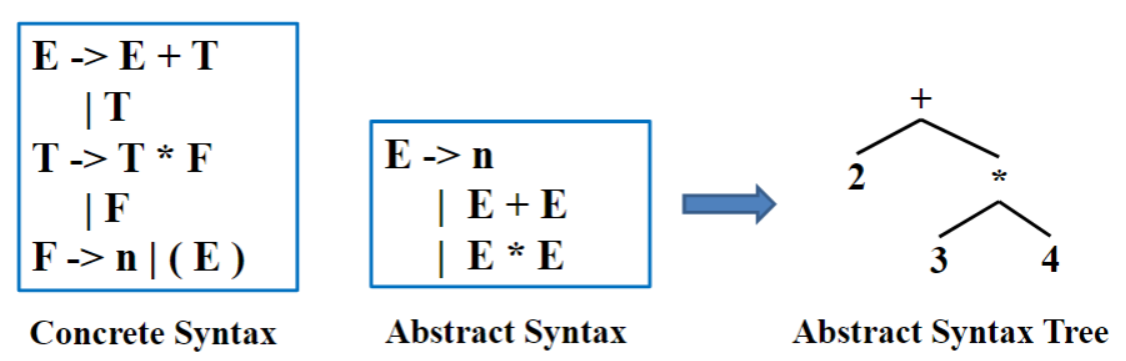
\includegraphics[width=0.88\linewidth]{pic/CP45/生成 AST}
    \caption{生成 AST}
\end{figure}

\subsection{Positions}
AST每个节点记录自己在源文件中的位置, 标记自己是具体哪几个字符派生而来的. 

\section{Semantic Analysis}
\subsection{Symbol Table(符号表)}

\begin{itemize}
    \item Binding:  把类型、值等信息绑定到一个identifier上
    \item Environment: 一些绑定的集合, 体现了程序当前环境下已声明的一些变量/函数/$\dots$
\end{itemize}


符号表就是Environment的一种实现方式. 
\begin{code}
    \caption{A Fancier Symbol Table}
    \begin{minted}{c++}
        enter_scope()   // start a new nested scope
        find_symbol(x)  // finds current x (or null)
        add_symbol(x)   // add a symbol x to the table
        check_scope(x)  // true if x defined in current scope
        exit_scope()    // exit current scope
    \end{minted}
\end{code}

符号表的实现:
\begin{itemize}
    \item Imperative(命令式): 插入 identifiers 时插入到头部, 在退出 scope 时方便 pop.  e.g. bucket list(hash table)
    \item Functional(函数式): 使用可持久化维护数据结构的历史, 退出 scope 时回到相应的历史状态即可. e.g. 可持久化二叉搜索树(persistent BST)
\end{itemize}